% Digital Logic Report Template
% Created: 2020-01-10, John Miller

%==========================================================
%=========== Document Setup  ==============================

% Formatting defined by class file
\documentclass[11pt]{article}

% ---- Document formatting ----
\usepackage[margin=1in]{geometry}	% Narrower margins
\usepackage{booktabs}				% Nice formatting of tables
\usepackage{graphicx}				% Ability to include graphics

%\setlength\parindent{0pt}	% Do not indent first line of paragraphs 
\usepackage[parfill]{parskip}		% Line space b/w paragraphs
%	parfill option prevents last line of pgrph from being fully justified

% Parskip package adds too much space around titles, fix with this
\RequirePackage{titlesec}
\titlespacing\section{0pt}{8pt plus 4pt minus 2pt}{3pt plus 2pt minus 2pt}
\titlespacing\subsection{0pt}{4pt plus 4pt minus 2pt}{-2pt plus 2pt minus 2pt}
\titlespacing\subsubsection{0pt}{2pt plus 4pt minus 2pt}{-6pt plus 2pt minus 2pt}

% ---- Hyperlinks ----
\usepackage[colorlinks=true,urlcolor=blue]{hyperref}	% For URL's. Automatically links internal references.

% ---- Code listings ----
\usepackage{listings} 					% Nice code layout and inclusion
\usepackage[usenames,dvipsnames]{xcolor}	% Colors (needs to be defined before using colors)

% Define custom colors for listings
\definecolor{listinggray}{gray}{0.98}		% Listings background color
\definecolor{rulegray}{gray}{0.7}			% Listings rule/frame color

% Style for Verilog
\lstdefinestyle{Verilog}{
	language=Verilog,					% Verilog
	backgroundcolor=\color{listinggray},	% light gray background
	rulecolor=\color{blue}, 			% blue frame lines
	frame=tb,							% lines above & below
	linewidth=\columnwidth, 			% set line width
	basicstyle=\small\ttfamily,	% basic font style that is used for the code	
	breaklines=true, 					% allow breaking across columns/pages
	tabsize=3,							% set tab size
	commentstyle=\color{gray},	% comments in italic 
	stringstyle=\upshape,				% strings are printed in normal font
	showspaces=false,					% don't underscore spaces
}

% How to use: \Verilog[listing_options]{file}
\newcommand{\Verilog}[2][]{%
	\lstinputlisting[style=Verilog,#1]{#2}
}




%======================================================
%=========== Body  ====================================
\begin{document}

\title{ELC 2137 Lab 10: 7-segment Display with Time-Division Multiplexing}
\author{Jake Simmons}

\maketitle


\section*{Summary}

Type the summary of your experiment and results here.  


\section*{Q\&A}

Answer questions posed in the lab assignment here.


\section*{Results}

\begin{figure}[ht]\centering
	\begin{tabular}{l|rrrrrrrrrrrrrrrrr}
		Time (ns): & 0 & 20 & 40 & 60 & 80  & 100 & 120 & 140 & 160 & 180 & 200 & 220 & 240 & 260 & 280  & 300 & 320  \\
		\midrule
		clk & 0 & 1 & 1 & 1 & 1 & 1 & 1 & 1 & 1 & 1 & 1 & 1 & 1 & 1 & 1 & 1 & 1 \\
		en & 0 & 1 & 1 & 1 & 0 & 0 & 1 & 0 & 1 & 0 & 1 & 1 & 0 & 1 & 1 & 1 & 1 \\
		rst & 0 & 1 & 0 & 0 & 0 & 0 & 0 & 0 & 0 & 0 & 0 & 0 & 0 & 0 & 0 & 0 & 0 \\
		\midrule
		W1 & X & 1 & 2 & 3 & 4 & 5 & 6 & 7 & 8 & 9 & a & b & c & d & e & f & 0 \\
		W2 & X & 0 & 0 & 0 & 0 & 0 & 0 & 0 & 0 & 0 & 0 & 0 & 0 & 0 & 0 & 1 & 0\\
		\bottomrule
	\end{tabular}\medskip
	
	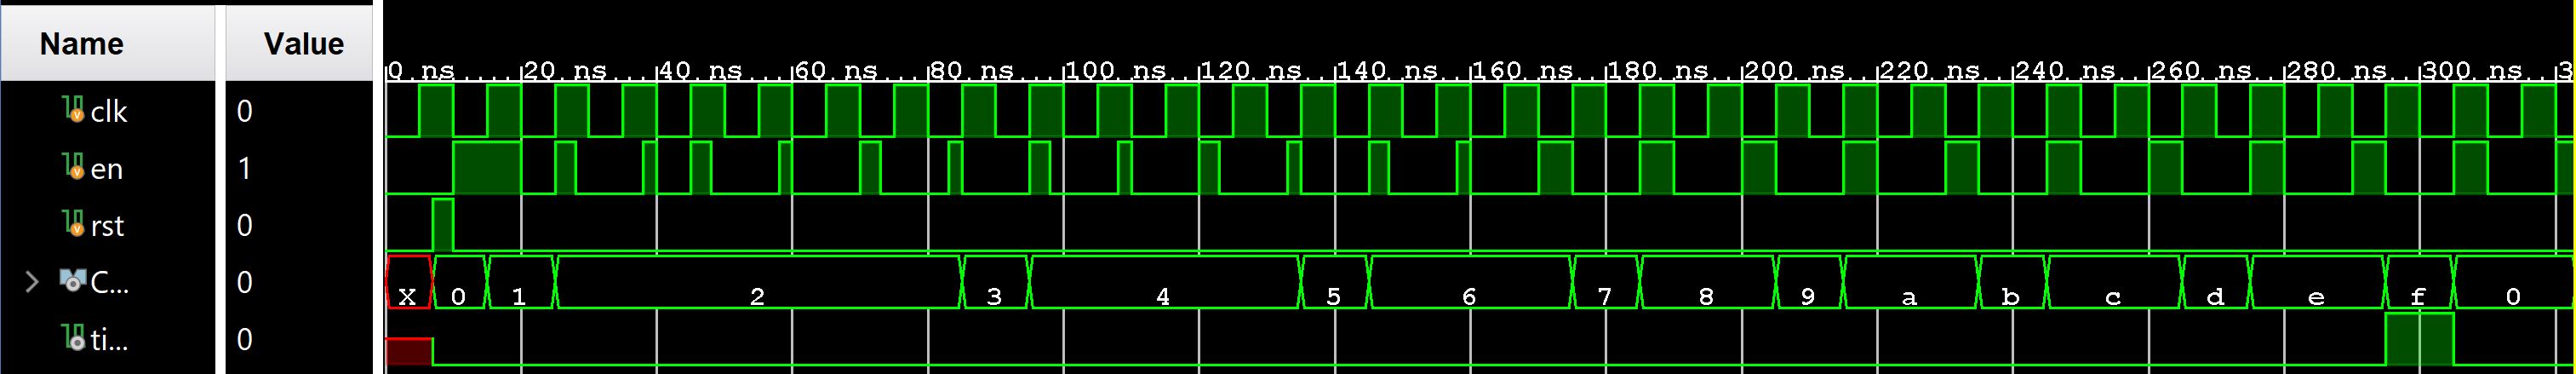
\includegraphics[width=1.15 \textwidth]{Counter_Test.JPG}
	\caption{Counter simulation waveform and ERT}
	\label{fig:sim_with_table}
\end{figure}

\begin{figure}[ht]\centering
	\begin{tabular}{l|rrrrrrrrrrrrrrrrrrrrr}
		Time (ms): & 0 & 2 & 4 & 6 & 8  & 10 & 12 & 14 & 16 & 18 & 20 & 22 & 24 & 26 & 28  & 30 & 32 & 34 & 36 & 38 & 40  \\
		\midrule
		clk & 0 & 1 & 1 & 1 & 1 & 1 & 1 & 1 & 1 & 1 & 1 & 1 & 1 & 1 & 1 & 1 & 1 & 1 & 1 & 1 & 1 \\
		rst & 1 & 0 & 0 & 0 & 0 & 0 & 0 & 0 & 0 & 0 & 0 & 0 & 0 & 0 & 0 & 0 & 0 & 0 & 0 & 0 & 0 \\
		data & 0 & 1 & 1 & 2 & 3 & 4 & 4 & 5 & 6 & 7 & 8 & 8 & 9 & a & b & c & c & d & e & e & f\\
		hexdec & 0 & 1 & 1 & 1 & 1 & 1 & 1 & 1 & 1 & 1 & 1 & 0 & 0 & 0 & 0 & 1 & 1 & 1 & 0 & 0 & 0 \\
		\midrule
		seg & 0 & 0 & 0 & 0 & 0 & 0 & 0 & 0 & 0 & 0 & 0 & 1 & 1 & 1 & 1 & 1 & 1 & 1 & 0 & 0 & 0\\
		dp & 1 & 1 & 1 & 1 & 1 & 1 & 1 & 1 & 1 & 1 & 1 & 1 & 1 & 1 & 1 & 1 & 1 & 1 & 1 & 1 & 1\\
		an & e & e & e & e & e & d & d & d & 7 & 7 & 7 & e & e & e & d & d & d & b & b & b & 7\\
		\bottomrule
	\end{tabular}\medskip
	
	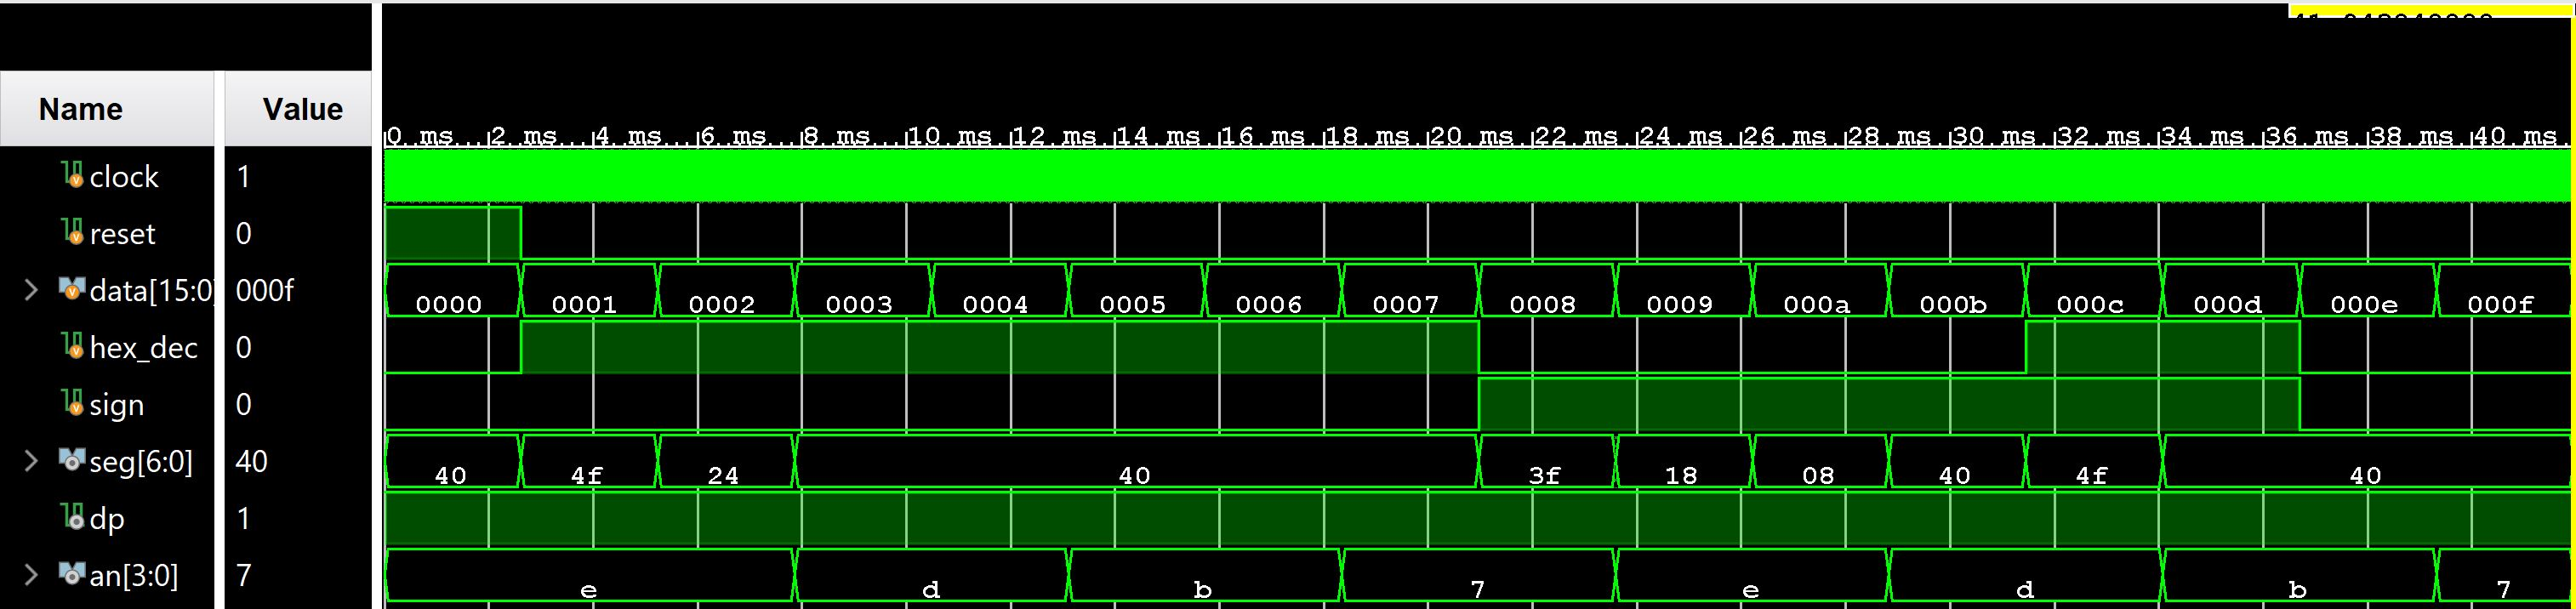
\includegraphics[width=1.15 \textwidth]{sseg4_TDM_Test.JPG}
	\caption{sseg4TDM simulation waveform and ERT}
	\label{fig:sim_with_table}
\end{figure}

\section*{Code}

Include all of the code you wrote or modified here.


\end{document}
